% This beamer template was adapted from "beamerthemeUppsala version 2008/05/15"
% for GSHS students, by Chinook Mok and GSHS TeX Society(http://latex.gs.hs.kr).
\documentclass[11pt]{beamer}
\hypersetup{pdfencoding=auto}

\usetheme{Berkeley}

\usepackage{xcolor}
\usepackage{amssymb,amsmath,graphicx}
\usepackage[spanish]{babel}
%\usepackage[hangul]{kotex}
\usepackage{multimedia}
\usepackage{setspace}
\usepackage{multicol}
%\usepackage{verbatim} %use 
\usepackage{lipsum}
\graphicspath{{images/}}
%% Footnote Setting %%

\let\oldfootnote\footnote
\renewcommand\footnote[1][]{\oldfootnote[frame,#1]}

\makeatletter % Makes maximum footnote counter of fnsymbol from 9 to 12.
\def\@fnsymbol#1{\ensuremath{\ifcase#1\or *\or \dagger\or \ddagger\or
		\mathsection\or \mathparagraph\or \|\or **\or \dagger\dagger
		\or \ddagger\ddagger\or \mathsection\mathsection
		\or \mathparagraph\mathparagraph \or \|\|\else\@ctrerr\fi}}
\makeatother
\renewcommand{\thefootnote}{\fnsymbol{footnote}}

%% Color Setting %%
\definecolor{Grey}{rgb}{0.6,0.6,0.6}
\definecolor{GSHSred}{RGB}{105,0,0}
\definecolor{GSHSblue}{RGB}{0,0,105}
\definecolor{GSHSRED}{RGB}{80,0,0}
\definecolor{GSHSBLUE}{RGB}{0,0,80}
\definecolor{gshsred}{RGB}{240,210,210}
\definecolor{gshsblue}{RGB}{210,210,240}
\setbeamercolor{title}{bg=white,fg=GSHSblue}
\setbeamercolor{author}{fg=GSHSblue}
\setbeamercolor{institute}{fg=GSHSblue}
\setbeamercolor{date}{fg=GSHSblue}
\setbeamercolor{logo}{bg=GSHSblue}
\setbeamercolor{sidebar}{bg=GSHSblue}
\setbeamercolor{frametitle}{bg=white,fg=GSHSblue}
\setbeamercolor{section in sidebar}{use=sidebar,bg=white,fg=sidebar.bg}
\setbeamercolor{subsection in sidebar}{parent=section in sidebar}
\setbeamercolor{subsubsection in sidebar}{parent=subsection in sidebar}
\setbeamercolor{item}{fg=GSHSblue}
\setbeamercolor{block title}{bg=GSHSBLUE,fg=white}
\setbeamercolor{block body}{bg=gshsblue,fg=black}

%% Frametitle Setting %%
\setbeamerfont{frametitle}{series=\bfseries}
\setbeamertemplate{frametitle}
{ \vspace*{-10mm}
  \leavevmode
  \hspace*{3pt}
  \begin{beamercolorbox}[wd=\paperwidth,ht=1ex,dp=1ex]{frametitle}
    \hspace*{7pt}\underline{\makebox[0.6\paperwidth][l]{
    \Large{\insertframetitle}}}
  \end{beamercolorbox}
}

             
%% Title Page Setting %%
\setbeamerfont{title}{series=\bfseries}
\setbeamertemplate{title page}{
  \vfill
  \vspace*{10mm}
  \raggedleft
  %% Title
  \usebeamerfont{title}\usebeamercolor[fg]{title}\inserttitle\par
  \vskip 2mm
  %% Subtitle
  \ifx\insertsubtitle\@empty
  \else\usebeamerfont{subtitle}\usebeamercolor[fg]{subtitle}\insertsubtitle
  \fi

  \vskip 3mm
  %% Horizontal line
  \usebeamercolor[fg]{title}\hrule height 2pt\hfill
  \vskip 10mm
  %% Author
  \usebeamercolor[fg]{author}\usebeamerfont{author}\insertauthor
  \vskip 1cm
  %% Institute
  \usebeamercolor[fg]{institute}\usebeamerfont{institute}\insertinstitute
  \vskip 1cm
  %% Date
  \usebeamercolor[fg]{date}\usebeamerfont{date}\insertdate
  \vfill
}

%% itemize bullet setting %%
\setbeamertemplate{itemize items}[ball]

%% block setting %%
\setbeamertemplate{blocks}[rounded][shadow=true]

%% caption setting %%
\setbeamertemplate{caption}[numbered]

%% Title, Author, Institute, Date %%
\title[]{Charla sobre seguridad inform\'atica}
\subtitle[]{C\'omo asegurar mi cuenta usando Google Authenticator}
\author[]{Se Hoon Park}
\date[]{\today}

%%%%%%%%%%%%%%%%%%%%%%%%%%%%%%%%%%%%%%%%%
% insert your own profile picture
%\logo{\includegraphics[width=15mm]{stackoverflow.pdf}}
%\logo{\includegraphics[width=8mm]{Profile_Picture.pdf}}

%% Main %%

\begin{document}

\begin{frame}[plain]
\titlepage
\end{frame}
\setbeamertemplate{sidebar left}[sidebar theme]

\setstretch{1.3} %줄간격


\section{Introducci\'on}
\begin{frame}{Proceso cl\'asico de logueo}\footnotesize
  \begin{block}{Qu\'e necesitamos para acceder a la cuenta?}
    \begin{itemize}
      \item<2-> Usuario Ej: fulano@gmail.com La parte que todo el mundo conoce
      \item<3-> Contrase\~na  esta parte se supone que solo uno sabe
    \end{itemize}
    \pause
    \pause
    \pause
    \color[rgb]{1,0,0} Qu\'e pasar\'ia si la contrase\~na fuera robada?
  \end{block}
\end{frame}
\begin{frame}{El peligro}
  \begin{figure}[ht]
    \begin{center}
      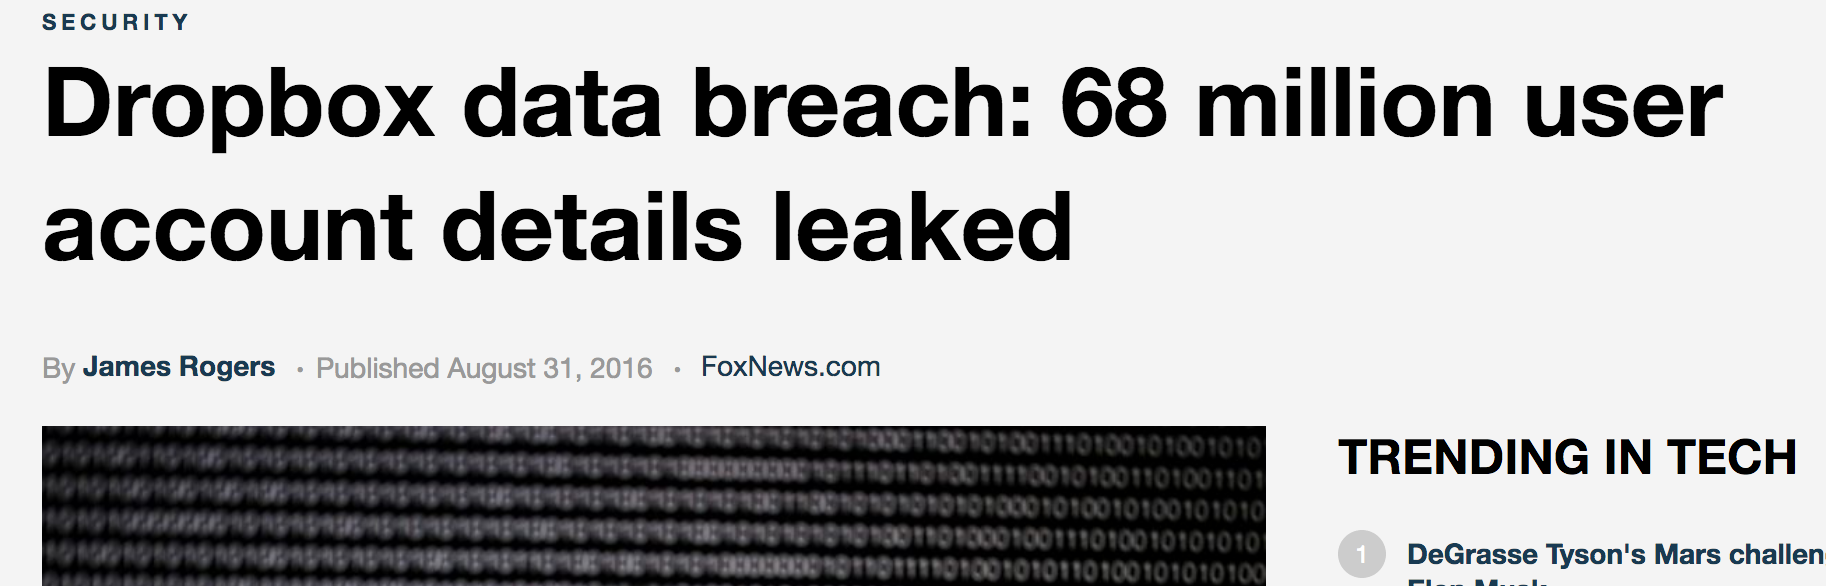
\includegraphics[width=4in]{noticia-dropbox.png}
	~\footnote{Qu\'e les parece tipo de noticias?}
    \end{center}
  \end{figure}
\end{frame}
\begin{frame}{base de datos de Dropbox filtrado}
  \begin{figure}[ht]
    \begin{center}
      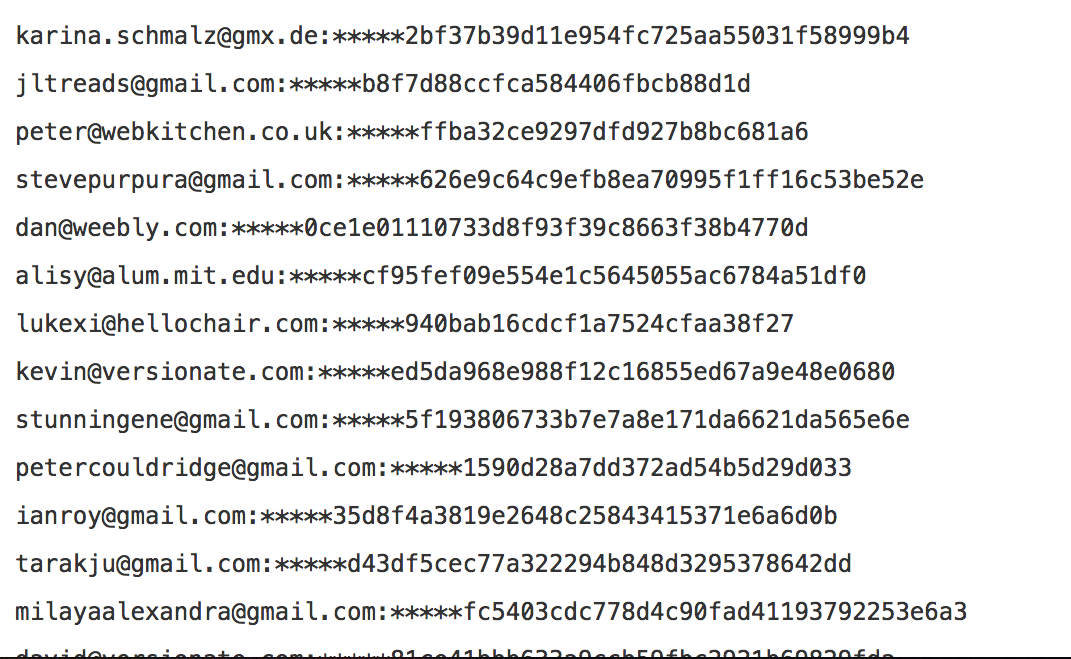
\includegraphics[height=2.75in, width=3in]{dropbox-database.png}
	~\footnote{Si aqu\'i incluye su cuenta, que har\'ia?}
    \end{center}
  \end{figure}
\end{frame}
\section{Verificaci\'on de 2 pasos}
\begin{frame}{Logueo va a ser diferente}
  \begin{figure}
    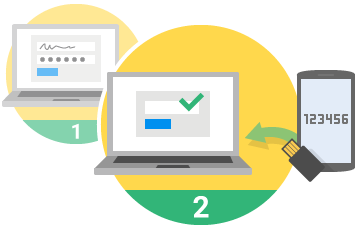
\includegraphics[width=4in]{how-works-img-1.png}
  \end{figure}
\end{frame}
\begin{frame}{Agrega una capa m\'as de seguridad}
  \begin{figure}
    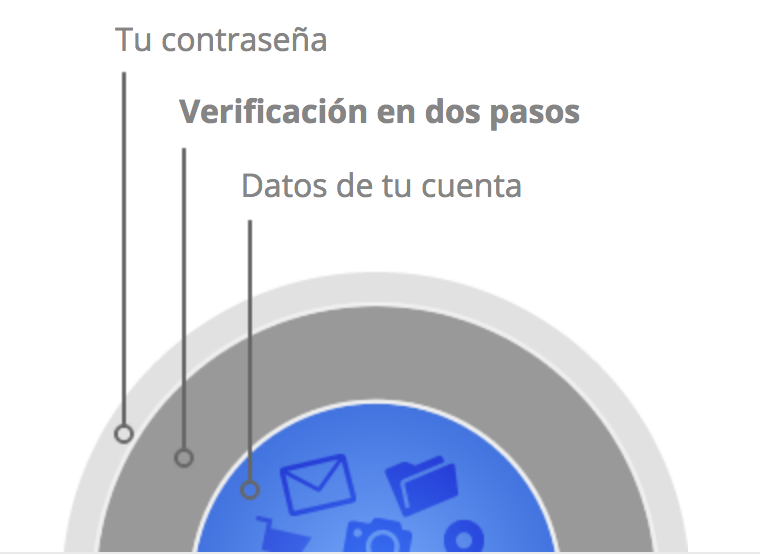
\includegraphics[width=4in]{unacapamas.png}
  \end{figure}
\end{frame}
\begin{frame}{Algo que sabes y algo que ten\'es}
  \begin{figure}
    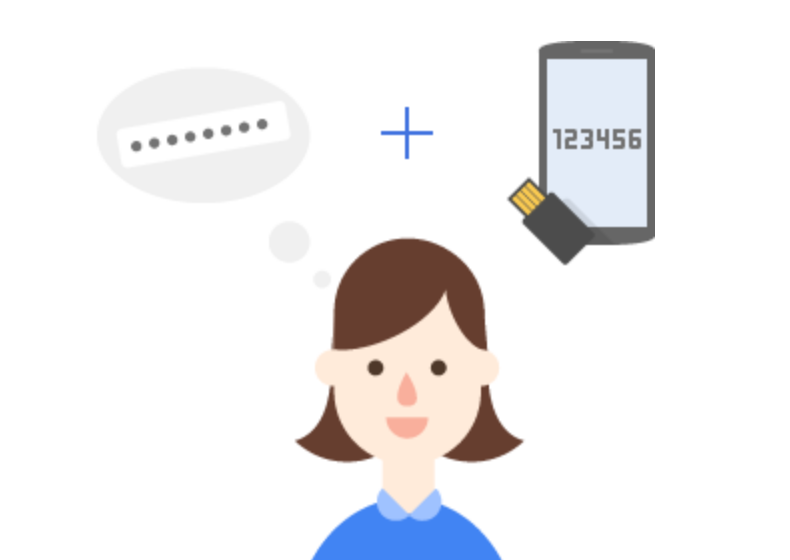
\includegraphics[width=4in]{algoqsabesyalgoqtenes.png}
  \end{figure}
\end{frame}
\begin{frame}{clave para un solo uso}
  \begin{block}{Qu\'e es?}
    OTP: One Time Password o contrase\~na para un solo uso\\
    Consiste en 6 d\'igitos\\
    Cuando configura verificaci\'on de 2 pasos, Google se encarga mandar via
    mensaje de texto o mensaje de voz
  \end{block}
\end{frame}
\section{C\'omo activarlo?}
\begin{frame}{Configurar Verificaci\'on de 2 pasos}
  \begin{block}{URL}
    https://myaccount.google.com/signinoptions/two-step-verification
  \end{block}
\end{frame}
\begin{frame}{1er paso}
  \begin{figure}
    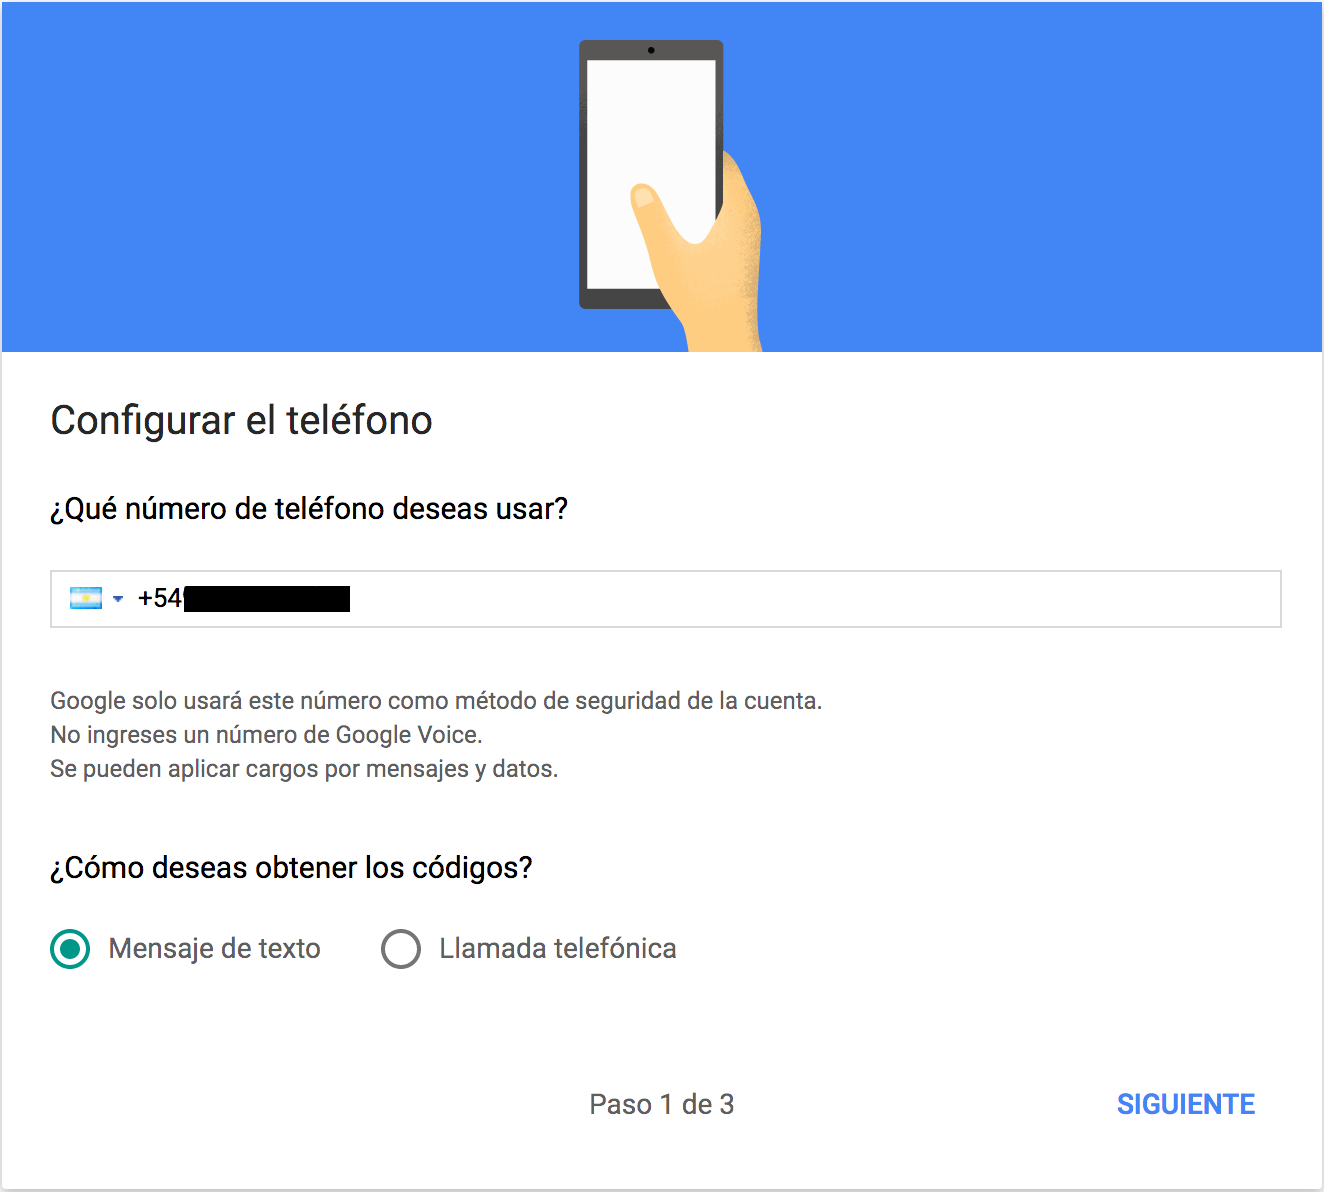
\includegraphics[width=3.25in]{1paso.png}
  \end{figure}
\end{frame}
\begin{frame}{2do paso}
  \begin{figure}
    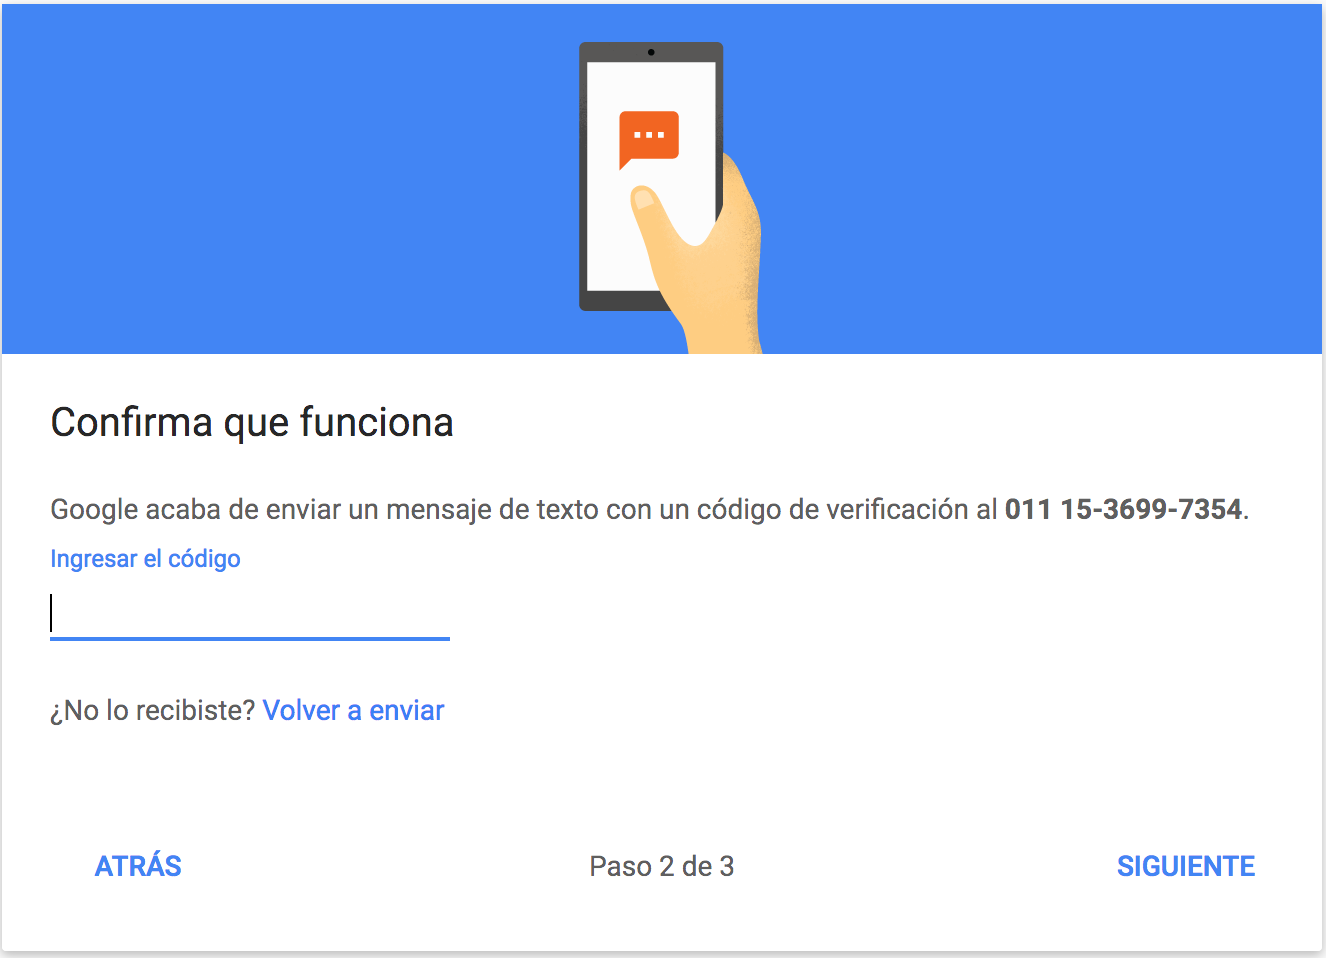
\includegraphics[width=3.25in]{2paso.png}
  \end{figure}
\end{frame}
\begin{frame}{3er paso}
  \begin{figure}
    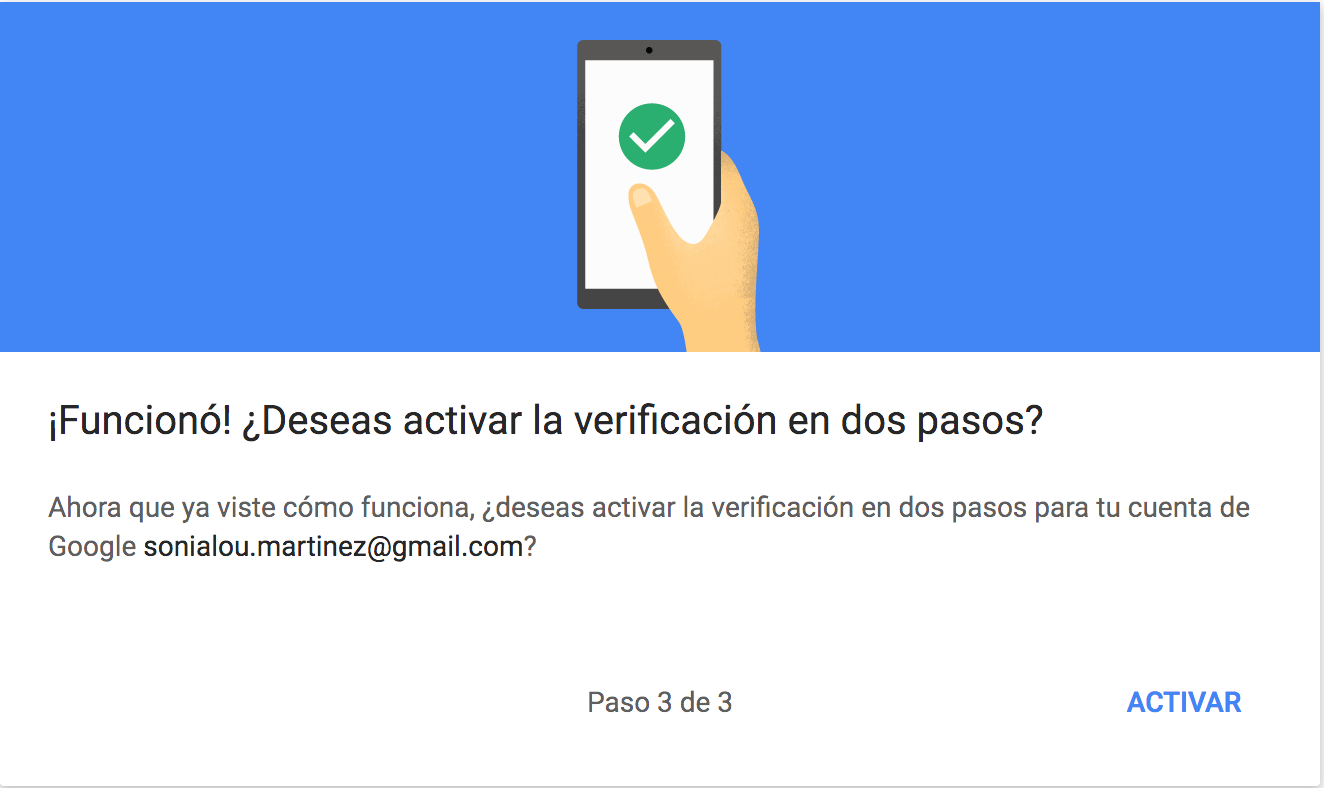
\includegraphics[width=3.25in]{3paso.png}
  \end{figure}
\end{frame}
\section{Desventaja}
\begin{frame}{Problema}
  \begin{block}{Qu\'e pasar\'ia si no estoy en condicion de recibir clave via mensaje?}
    Por ej. Estoy en otro pa\'is. \\
    \color[rgb]{1,0,0} La \'unica soluci\'on ser\'ia roaming?
  \end{block}
\end{frame}
\section{Google Authenticator}
\begin{frame}{Google Authenticator}
  \begin{figure}
    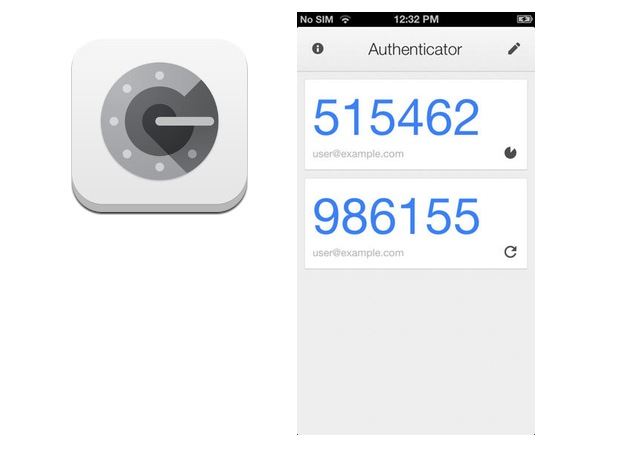
\includegraphics[width=4in]{google-authenticator.jpg}
  \end{figure}
\end{frame}
\begin{frame}{Generar OTP en mi smartphone}
  \begin{block}{Via Google Authenticator}
    Google Authenticator genera contrase\~na un solo uso cada 30 segundos\\
    O sea, no necesita m\'as recibir OTP via mensaje
  \end{block}
\end{frame}
\begin{frame}{D\'onde configurar para usar G.A?}
  \begin{block}{URL}
    https://myaccount.google.com/signinoptions/two-step-verification
  \end{block}
\end{frame}
\begin{frame}{fijese d\'onde}
  \begin{figure}
    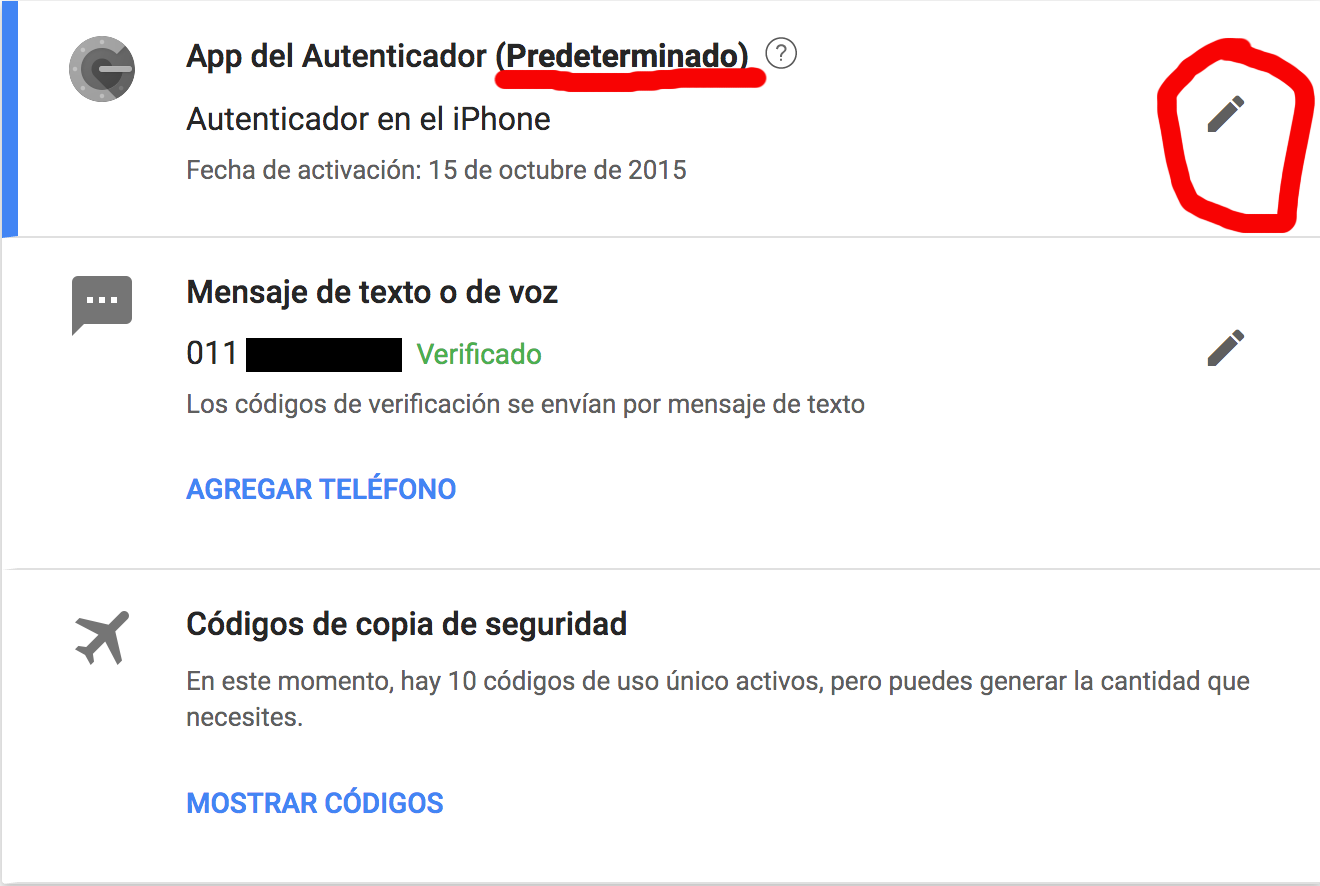
\includegraphics[width=4in]{2wayauth.png}
  \end{figure}
\end{frame}
\begin{frame}{As\'i habilita el uso de G.A.}
  \begin{figure}{Hay que escanear el c\'odigo QR usando G.A.}
    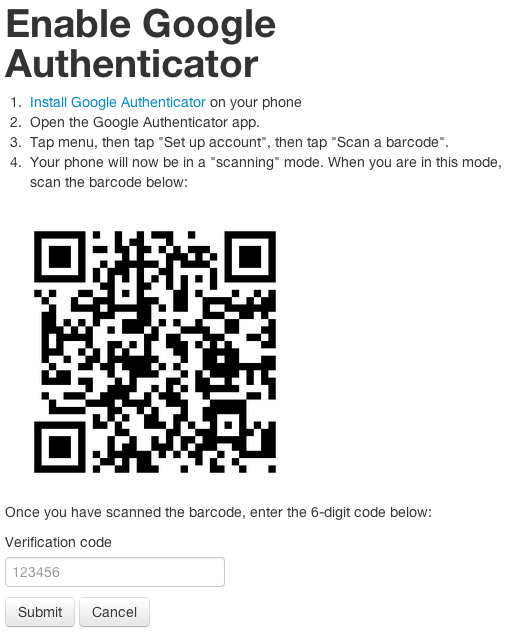
\includegraphics[width=2in]{enable-authenticator.png}
  \end{figure}
\end{frame}
\section{C\'odigos de copia de seguridad}
\begin{frame}{C\'odigos de copia de seguridad}
  \begin{block}{Claves de emergencia}
    \begin{itemize}
      \item Son 10 c\'odigos de 8 d\'igitos para el uso de emergencia.
      \item Por ej. si perdi\'o el celular y no hay forma de acceder a la cuenta. Hay que usar estos c\'odigos de un solo uso. 
      \item Hay que bajarlo y *mejor* tenerlo impreso en alg\'un lugar seguro.
      \item Se puede generar cuantas veces quiera pero las claves ya usadas habr\'ia que tachar para indicar que ya fue usado
    \end{itemize}
  \end{block}
\end{frame}
\section{contrase\~nas de aplicaci\'on}
\begin{frame}{Contrase\~nas de aplicaci\'on}
  \begin{block}{Por qu\'e y Para qu\'e?}
    \begin{itemize}
    	\item Es muy probable que las aplicaciones que accedan a la cuenta configurada recientemente va a mostrar error de contrase\~na incorrecta Por ej. Outlook
    	\item Habr\'ia que configuar que use una clave para aplicacion o dispositivo para ese caso
    	\item Consiste en una clave de 16 d\'igitos. Una clave generada para la aplicaci\'on o el dispositivo
    	\item https://myaccount.google.com/apppasswords 
    	\item Para m\'as informaci\'on https://support.google.com/accounts/answer/185833
    \end{itemize}
  \end{block}
\end{frame}
\section{Los servicios que soportan 2WA}
\begin{frame}
  \begin{block}{Los sitios que soportan 2WA}
    \begin{itemize}
      \item Google
      \item Facebook
      \item Dropbox
      \item Hotmail
      \item Github
      \item Slack
      \item Snapchat
      \item Etc.
    \end{itemize}
  \end{block}
\end{frame}
\begin{frame}
  \begin{block}{Si quieren bajar esta prensentaci\'on}
    http://j.mp/2o6Khkq
  \end{block}
\end{frame}
\begin{frame}{https://logosklogos.com}
  \begin{figure}{Biblia interlineal}
    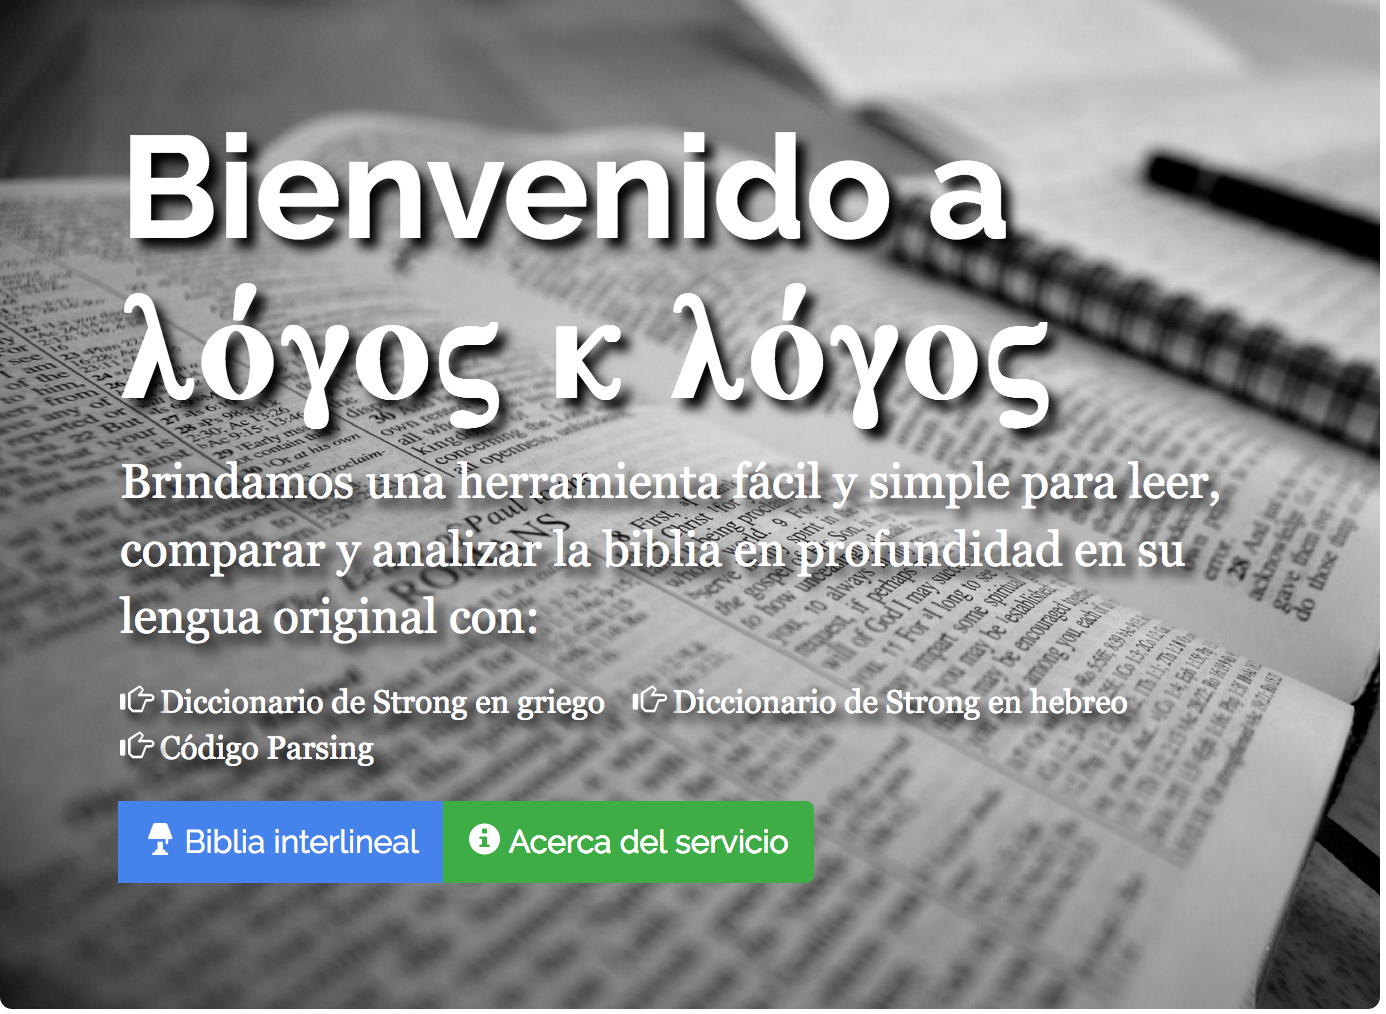
\includegraphics[width=3.25in]{logos-home.png}
  \end{figure}
\end{frame}
\begin{frame}{https://logosklogos.com}
  \begin{figure}{Nuevo testamento}
    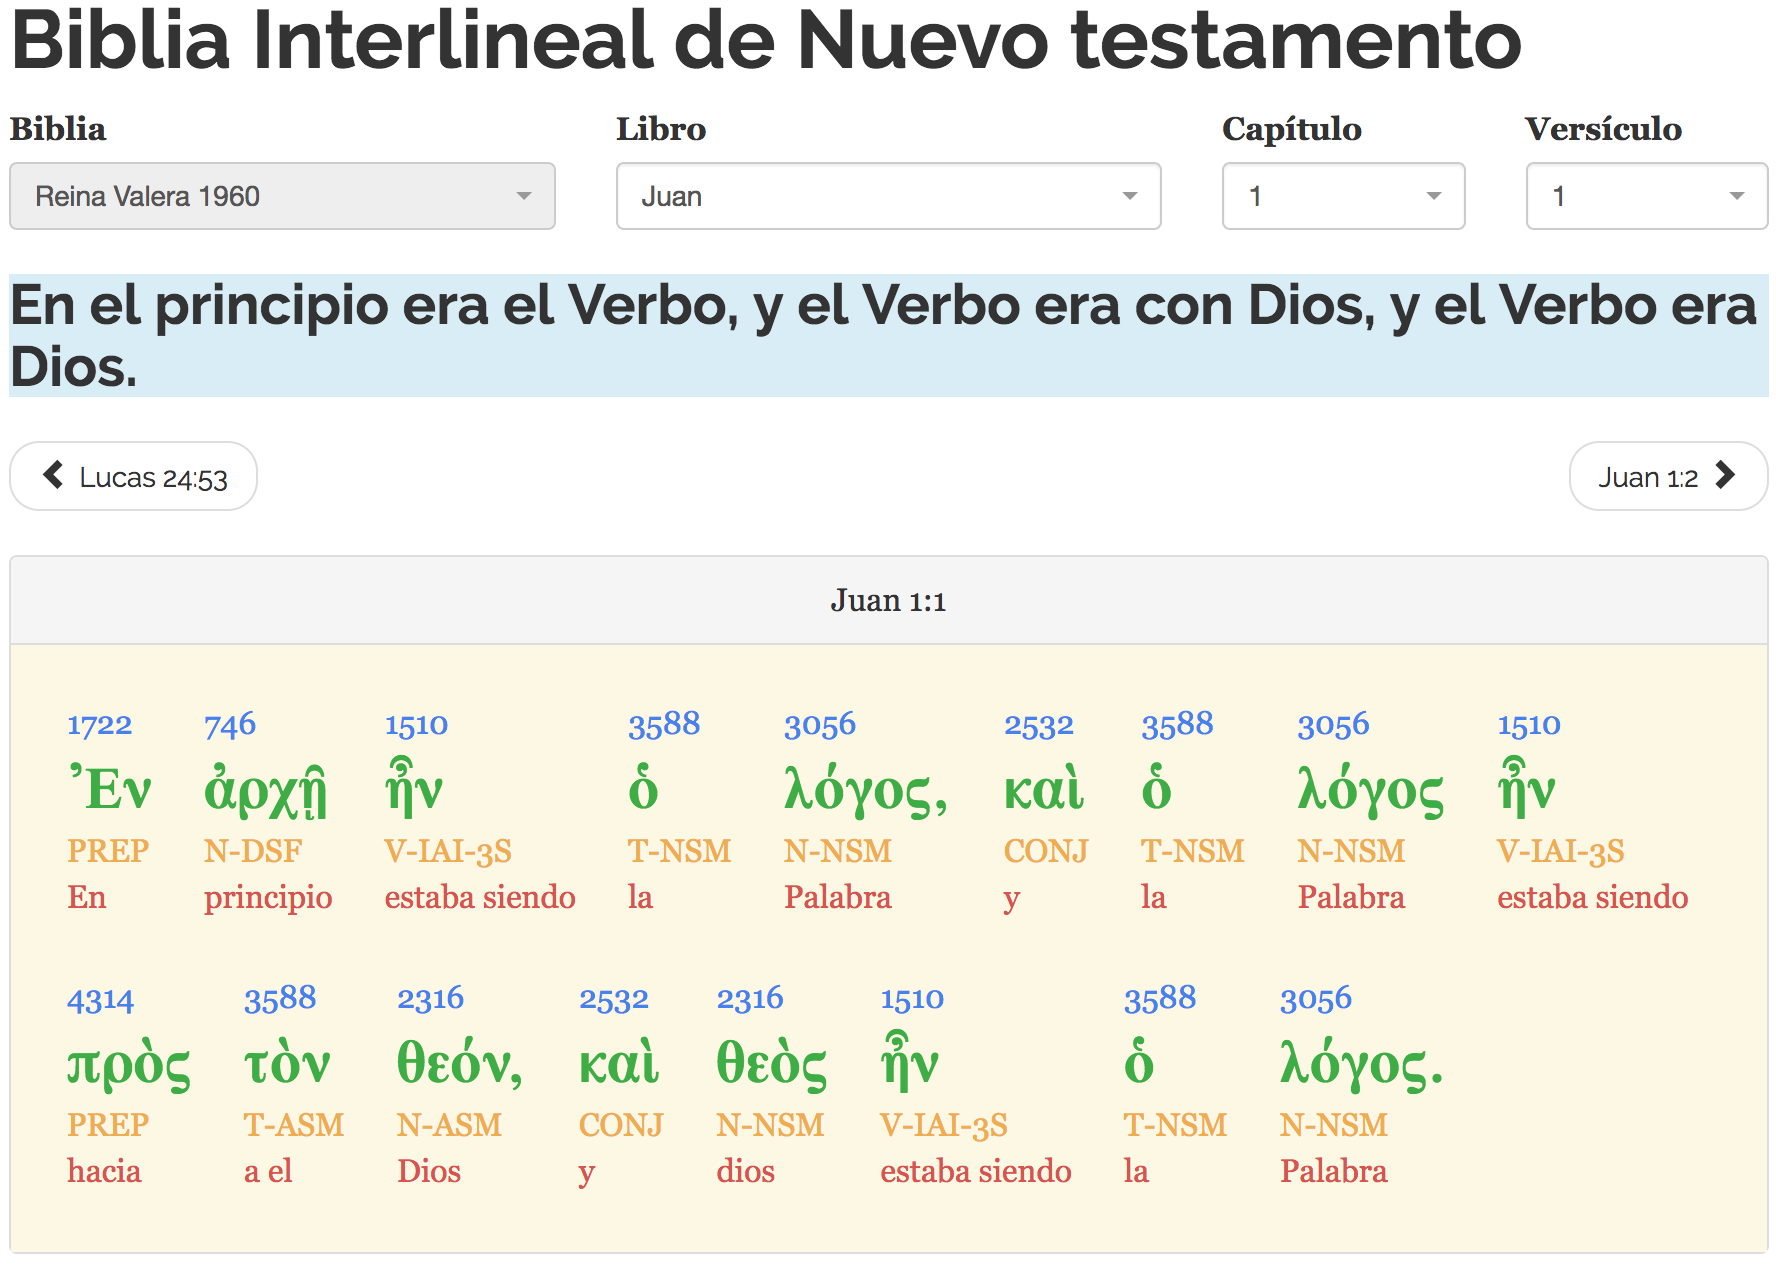
\includegraphics[width=3.25in]{logos-griego.png}
  \end{figure}
\end{frame}
\begin{frame}{https://logosklogos.com}
  \begin{figure}{Antiguo testamento}
    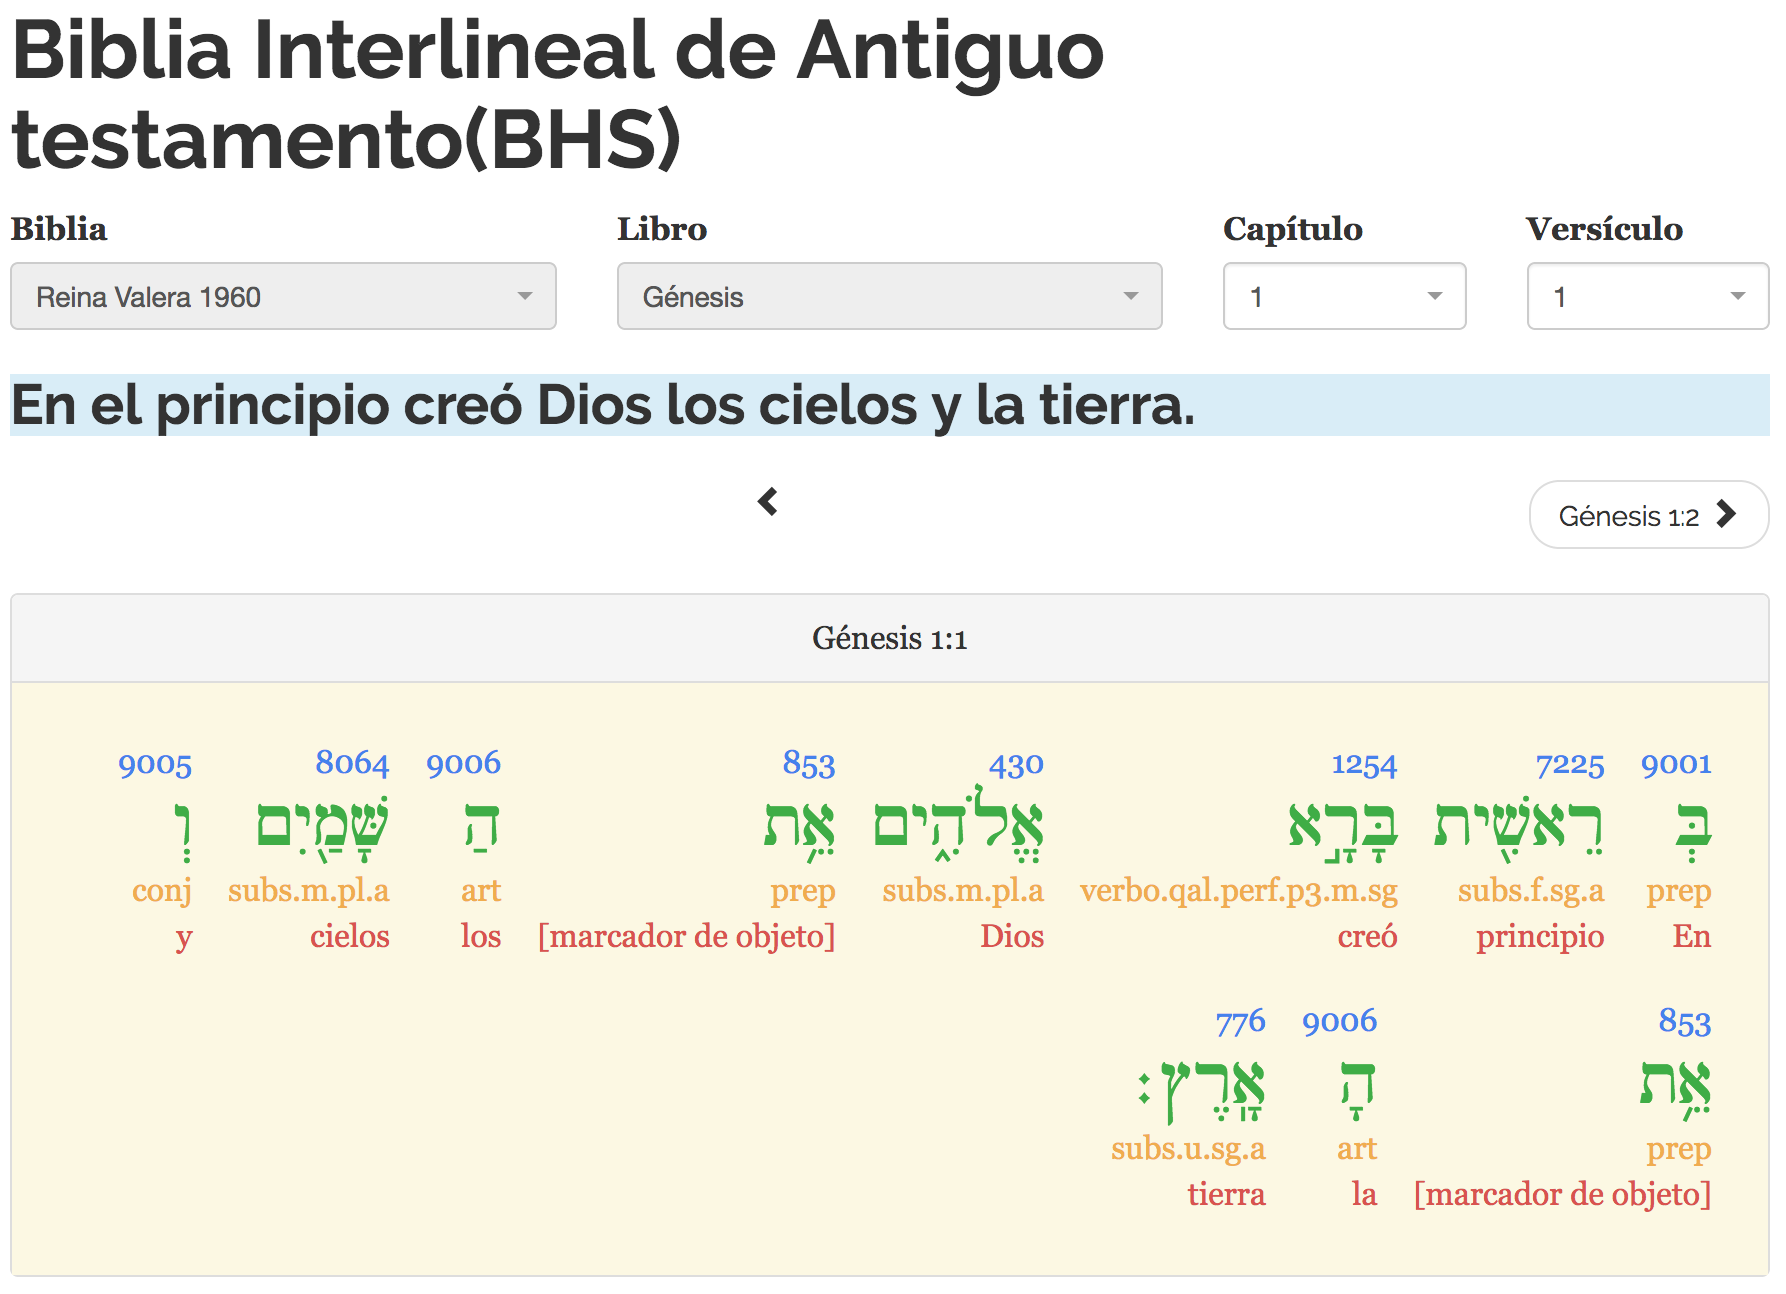
\includegraphics[width=3.25in]{logos-hebreo.png}
  \end{figure}
\end{frame}
\end{document}
